



\chapter{Vecteurs et repérage}


\section{Repère du plan}
\begin{minipage}[c]{0.65\linewidth}
\noindent Trois points distincts deux à deux $O$, $I$ et $J$ du plan forment un repère, que l'on peut noter $(O,I,J)$.\\
L'origine $O$ et les unités $OI$ et $OJ$ permettent de graduer les axes $(OI)$ et $(OJ)$.\\
Si on pose $\overrightarrow{i}=\overrightarrow{OI}$ et $\overrightarrow{j}=\overrightarrow{OJ}$, alors ce repère se note aussi $(O,\overrightarrow{i},\overrightarrow{j})$.
\end{minipage} \hfill
\begin{minipage}[c]{0.26\linewidth}
\begin{center}
\begin{tikzpicture}[scale=0.8]
    % Grille en pointillés
    \draw[dotted, gray] (-3,-3) grid (3,3);
    
    % Axes principaux
    \draw[->, thick] (-3,0) -- (3,0) node[right] {};
    \draw[->, thick] (0,-3) -- (0,3) node[above] {};
    
    % Points et labels
    \node[below left] at (0,0) {$O$};
    \node[below] at (1,0) {$I$};
    \node[above left] at (0,1) {$J$};
    
    % Vecteurs
    \draw[->, very thick, Couleur6] (0,0) -- (1,0) node[midway, below] {$\vec{i}$};
    \draw[->, very thick, Couleur6] (0,0) -- (0,1) node[midway, left] {$\vec{j}$};
\end{tikzpicture}
\end{center}
\end{minipage}




\begin{Définition} $ $
\begin{itemize}[label=\textcolor{Couleur6}{$\bullet$}]
\item On appelle {\bf{repère du plan}} tout triplet $(O,\overrightarrow{i},\overrightarrow{j})$, où $O$ est un point et $\overrightarrow{i}$ et $\overrightarrow{j}$ sont deux vecteurs non colinéaires.
\item Un repère est dit {\bf{orthogonal}} si $\overrightarrow{i}$ et $\overrightarrow{j}$ ont des directions perpendiculaires.
\item Un repère est dit {\bf{orthonormé}} s'il est orthogonal et si $\overrightarrow{i}$ et $\overrightarrow{j}$ sont de norme $1$.
\end{itemize}

\end{Définition}

\begin{center}
\begin{tikzpicture}

% Premier repère : orthogonal
\begin{scope}[xshift=-6cm]
    \node[above] at (0,2.5) {\textbf{Repère orthogonal}};
    
    % Axes
    \draw[->, thick] (-1.5,0) -- (2,0);
    \draw[->, thick] (0,-1.5) -- (0,2);
    
    % Vecteurs de base
    \draw[->, very thick, Couleur6] (0,0) -- (0.8,0) node[midway, below] {$\vec{i}$};
    \draw[->, very thick, Couleur6] (0,0) -- (0,1.5) node[midway, left] {$\vec{j}$};
    
    % Origine
    \node[below left] at (0,0) {$0$};
\end{scope}

% Deuxième repère : orthonormé
\begin{scope}
    \node[above] at (0,2.5) {\textbf{Repère orthonormé}};
    
    % Axes
    \draw[->, thick] (-1.5,0) -- (2,0);
    \draw[->, thick] (0,-1.5) -- (0,2);
    
    % Vecteurs de base (même longueur)
    \draw[->, very thick, Couleur6] (0,0) -- (0.8,0) node[midway, below] {$\vec{i}$};
    \draw[->, very thick, Couleur6] (0,0) -- (0,0.8) node[midway, left] {$\vec{j}$};
    
    % Origine
    \node[below left] at (0,0) {$0$};
\end{scope}

% Troisième repère : quelconque
\begin{scope}[xshift=6cm]
    \node[above] at (0,2.5) {\textbf{Repère quelconque}};
    
    % Axes obliques
    \draw[->, thick] (-1.5,0) -- (2,0);
    \draw[->, thick] (-1,-1) -- (1.5,1.5);
    
    % Vecteurs de base
    \draw[->, very thick, Couleur6] (0,0) -- (1,0) node[midway, below] {$\vec{i}$};
    \draw[->, very thick, Couleur6] (0,0) -- (0.7,0.7) node[midway, above left] {$\vec{j}$};
    
    % Origine
    \node[below left] at (0.2,0) {$0$};
\end{scope}

\end{tikzpicture}
\end{center}






\subsection{Coordonnées d'un vecteur}

\begin{Définition} $ $ \\
\begin{minipage}[c]{0.6\linewidth}
Soit $M$ un point quelconque d'un repère $(O,\overrightarrow{i},\overrightarrow{j})$ et un vecteur $\overrightarrow{u}$ tel que $\overrightarrow{OM}=\overrightarrow{u}$.\\
Les {\bf{coordonnées du vecteur}} $\overrightarrow{u}$ sont les coordonnées du point $M$ à savoir $(x_M,y_M)$.\\
On note $\overrightarrow{u}\begin{pmatrix} 
 x_M \\ 
y_M
 \end{pmatrix}$.\\
On a $\overrightarrow{OM}=x_M\overrightarrow{i}+y_M\overrightarrow{j}$.
\end{minipage} \hfill
\begin{minipage}[c]{0.36\linewidth}
\begin{center}
\begin{tikzpicture}[scale=0.8]
    % Grille en pointillés
    \draw[dotted, gray] (-3,-2) grid (5,5);
    
    % Axes principaux
    \draw[->, thick] (-3,0) -- (5,0) node[left, below] {$x$};
    \draw[->, thick] (0,-2) -- (0,5) node[left] {$y$};
    
    % Origine et vecteurs de base
    \node[below left] at (0,0) {$O$};
    \draw[->, thick, Couleur6] (0,0) -- (1,0) node[midway, below] {$\vec{i}$};
    \draw[->, thick, Couleur6] (0,0) -- (0,1) node[midway, left] {$\vec{j}$};
    
    % Vecteur u
    \draw[->, very thick, Couleur8] (-2,2) -- (2,4);
    \node[Couleur8] at (-0.5,3.2) {$\vec{u}$};
    

\end{tikzpicture}
\end{center}
\end{minipage}

\end{Définition}

\newpage
\begin{Méthode}Déterminer les coordonnées d'un vecteur par lecture graphique. \\
Déterminer les coordonnées des vecteurs $\overrightarrow{AB}$, $\overrightarrow{CD}$, $\overrightarrow{EF}$ par lecture graphique : \begin{center}
\begin{tikzpicture}[scale=0.6]
    % Grille en pointillés
    \draw[dotted, gray] (-4,-6) grid (7,5);
    
    % Axes principaux
    \draw[->, thick] (-4,0) -- (7,0) node[right] {$x$};
    \draw[->, thick] (0,-6) -- (0,5) node[above] {$y$};
    
    % Origine et vecteurs de base
    \node[below left] at (0,0) {$O$};
    \draw[->, thick, Couleur6] (0,0) -- (1,0) node[midway, below] {$\vec{i}$};
    \draw[->, thick, Couleur6] (0,0) -- (0,1) node[midway, left] {$\vec{j}$};
    
    % Points
    \fill[Couleur8] (1,1) circle (0pt) node[left, Couleur8] {$A$};
    \fill[Couleur8] (5,4) circle (0pt) node[right, Couleur8] {$B$};
    \fill[Couleur8] (-1,-2) circle (0pt) node[right, Couleur8] {$C$};
    \fill[Couleur8] (-3,3) circle (0pt) node[right, Couleur8] {$D$};
    \fill[Couleur8] (2,-5) circle (0pt) node[left, Couleur8] {$E$};
    \fill[Couleur8] (6,-2) circle (0pt) node[right, Couleur8] {$F$};
    
    % Vecteurs principaux
    \draw[->, very thick, Couleur8] (1,1) -- (5,4);   % AB
    \draw[->, very thick, Couleur8] (-1,-2) -- (-3,3);  % CD
    \draw[->, very thick, Couleur8] (2,-5) -- (6,-2);  % EF
    
    % Lignes de construction et projections
    \draw[->,thick, Couleur3] (1,1) -- (5,1);
    \draw[->,thick, Couleur3] (5,1) -- (5,4);

    \draw[->,thick, Couleur3] (-1,-2) -- (-3,-2);
    \draw[->,thick, Couleur3] (-3,-2) -- (-3,3);
    
        \draw[->,thick, Couleur3] (2,-5) -- (6,-5);
    \draw[->,thick, Couleur3] (6,-5) -- (6,-2);
    
    % Annotations des coordonnées en vert
    \node[Couleur3] at (3,0.5) {$+4$};
    \node[Couleur3] at (5.4,2.3) {$+3$};
    
    \node[Couleur3] at (-2,-2.5) {$-2$};
    \node[Couleur3] at (-3.5,0.3) {$+4$};
    
    \node[Couleur3] at (4.5,-5.5) {$+4$};
    \node[Couleur3] at (6.5,-3.5) {$+3$};

    
\end{tikzpicture}

\end{center}
Pour aller de $A$ vers $B$, on effectue une translation de $4$ carreaux vers la droite $(+4)$\\ et une translation de $3$ carreaux vers le haut  $(+3)$. \\
On trace ainsi un \og chemin \fg{} de vecteurs $\overrightarrow{i}$ et $\overrightarrow{j}$ mis bout à bout reliant l'origine et l'extrémité du vecteur $\overrightarrow{AB}$. \\
Ainsi, $\overrightarrow{AB}=4\overrightarrow{i}+3\overrightarrow{j}$. Les coordonnées de $\overrightarrow{AB}$ sont donc $\begin{pmatrix} 
4 \\ 
3
 \end{pmatrix}$. \\
 De même, $\overrightarrow{CD}\begin{pmatrix} 
-2 \\ 
5
 \end{pmatrix}$ et $\overrightarrow{EF}\begin{pmatrix} 
4 \\ 
3
 \end{pmatrix}$.
 

\end{Méthode}



\begin{Propriété}
Soit $A$ et $B$ deux points de coordonnées $(x_A,y_A)$ et $(x_B,y_B)$ dans un repère $(O,\overrightarrow{i},\overrightarrow{j})$.\\
Le vecteur $\overrightarrow{AB}$ a pour coorodonnées $\begin{pmatrix} 
x_B-x_A \\ 
y_B-y_A
 \end{pmatrix}$.
\end{Propriété}

\begin{Méthode}Déterminer les coordonnées d'un vecteur par calcul. \\
Soit $A(1;1)$, $B(5;4)$, $C(-1;-2)$, $D(-3;3)$, $E(2;-5)$ et $F(6;-2)$.\\
Déterminer les coordonnées des vecteurs $\overrightarrow{AB}$, $\overrightarrow{CD}$ et $\overrightarrow{EF}$.\\
$\overrightarrow{AB}\begin{pmatrix} 
x_B-x_A \\ 
y_B-y_A
 \end{pmatrix}=\begin{pmatrix} 
5-1 \\ 
4-1
 \end{pmatrix}=\begin{pmatrix} 
4 \\
3
 \end{pmatrix}$, 
$\overrightarrow{CD}\begin{pmatrix} 
-3-(-1) \\ 
3-(-2)
 \end{pmatrix}=\begin{pmatrix} 
-2 \\
5
 \end{pmatrix}$, $\overrightarrow{EF}\begin{pmatrix} 
6-2 \\ 
-2-(-5)
 \end{pmatrix}=\begin{pmatrix} 
4 \\
3
 \end{pmatrix}$.



\end{Méthode}


\begin{Propriété} $ $ \\
Soit $\overrightarrow{u}$ et $\overrightarrow{v}$ deux vecteurs de coordonnées $\begin{pmatrix} 
x \\
y
 \end{pmatrix}$ et  $\begin{pmatrix} 
x' \\
y'
 \end{pmatrix}$ dans un repère $(O,\overrightarrow{i},\overrightarrow{j})$ et un réel $k$.
\begin{itemize}[label=\textcolor{Couleur2}{$\bullet$}]

 \item $\overrightarrow{u}=\overrightarrow{v}$ équivaut à $x=x'$ et $y=y'$ autrement dit  $\overrightarrow{u}$ et $\overrightarrow{v}$ ont les mêmes coordonnées.
 \item Le vecteur $\overrightarrow{u}+\overrightarrow{v}$ a pour coordonnées $\begin{pmatrix} 
x+x' \\
y+y'
 \end{pmatrix}$.
 \item Le vecteur $k\overrightarrow{u}$ a pour coorodonnées $\begin{pmatrix} 
kx \\
ky
 \end{pmatrix}$.
 \end{itemize}

\end{Propriété}


\begin{Remarque}
Si $\overrightarrow{u}$ a pour coordonnées $\begin{pmatrix} 
x \\
y
 \end{pmatrix}$ alors $-\overrightarrow{u}$ a pour coordonnées $\begin{pmatrix} 
-x \\
-y
 \end{pmatrix}$.

\end{Remarque}

\paragraph{Retour sur la propriété coordonnées d'un vecteur.}


\begin{Méthode}Appliquer les formules sur les coordonnées des vecteurs. \\
En reprenant l'exemple précédent, calculer les coordonnées des vecteurs $4\overrightarrow{AB}$, $3\overrightarrow{CD}$, et $4\overrightarrow{AB}-3\overrightarrow{CD}$. \\

On a $\overrightarrow{AB}\begin{pmatrix} 
4 \\
3
 \end{pmatrix}$ et 
$\overrightarrow{CD}\begin{pmatrix} 
-2 \\
5
 \end{pmatrix}$.\\ Donc $4\overrightarrow{AB}\begin{pmatrix} 
4\times 4 \\
4\times 3
 \end{pmatrix}=\begin{pmatrix} 
16 \\
12
 \end{pmatrix}$ et $3\overrightarrow{CD}\begin{pmatrix} 
3\times -2 \\
3\times 5
 \end{pmatrix}=\begin{pmatrix} 
-6 \\
15
 \end{pmatrix}$. \\
 Enfin, $4\overrightarrow{AB}-3\overrightarrow{CD}\begin{pmatrix} 
16-(-6) \\
12-15
 \end{pmatrix}=\begin{pmatrix} 
22 \\
-3
 \end{pmatrix}$.

\end{Méthode}
\vspace{0.5cm}
\begin{Méthode}Calculer les coordonnées d'un point défini par une égalité vectorielle. \\
Dans un repère, soit les points $A(-1;2)$, $B(3;-4)$ et $C(-3,2)$.\\
Déterminer les coordonnées du point $D$ tel que $ABCD$ soit un parallélogramme. 
\\
$ABCD$ est un parallélogramme si et seulement si $\overrightarrow{AB}=\overrightarrow{DC}$. \\
On a $\overrightarrow{AB}\begin{pmatrix} 
-3-(-1) \\
-4-2
 \end{pmatrix}=\begin{pmatrix} 
-2 \\
-6
 \end{pmatrix}$ et $\overrightarrow{DC}\begin{pmatrix} 
-3-x_D \\
2-y_D
 \end{pmatrix}$. \\
 Donc $-3-x_D=-2$ et $2-y_D=-6$.\\
 Soit $x_D=-1$ et $y_D=8$. 
 
\end{Méthode}

\vspace{0.5cm}

\section{Colinéarité de deux vecteurs}
\subsection{Définitions et premières propriétés}
\vspace{0.5cm}
\begin{Définition}
Dire que deux vecteurs $\overrightarrow{u}$ et $\overrightarrow{v}$ sont colinéaires signifie qu'il existe un réel $k$ tel que $\overrightarrow{v}=k\overrightarrow{u}$.

\end{Définition}
\vspace{0.5cm}
\begin{Exemple}
\leavevmode\vspace{-\baselineskip}
\begin{center}

\begin{tikzpicture}[scale=0.8]
    % Grille en pointillés
    \draw[dotted, gray] (-3,-2) grid (5,5);
    
    % Axes principaux
    \draw[->, thick] (-3,0) -- (5,0) node[right] {$x$};
    \draw[->, thick] (0,-2) -- (0,5) node[above] {$y$};
    
    % Origine et vecteurs de base
    \node[below left] at (0,0) {$O$};
    \draw[->, thick, Couleur6] (0,0) -- (1,0) node[midway, below] {$\vec{i}$};
    \draw[->, thick, Couleur6] (0,0) -- (0,1) node[midway, left] {$\vec{j}$};
    
    % Vecteur u
    \draw[->, very thick, Couleur8] (2,1) -- (4,2);
    \node[above right, Couleur8] at (3.2,0.8) {$\vec{u}$};
    
    % Vecteur v = -3u
    \draw[->, very thick, Couleur8] (4,5) -- (-2,2);
    \node[above left, Couleur8] at (3,2.8) {$\vec{v} = -3\vec{u}$};

\end{tikzpicture}
\end{center}
On a $\overrightarrow{v}=-3\overrightarrow{u}$. \\
Donc $\overrightarrow{u}$ et $\overrightarrow{v}$ sont colinéaires.
\end{Exemple}


\begin{Remarque}
${\color{Couleur7}{\bullet}}$ Par convention, le vecteur $\overrightarrow{0}$ est colinéaire à tout vecteur du plan.\\
${\color{Couleur7}{\bullet}}$ Deux vecteurs $\overrightarrow{u}$ et $\overrightarrow{v}$ sont {\bf{colinéaires}} lorsqu'ils ont la {\bf{même direction}}.
\end{Remarque}




\newpage


\subsection{Critère de colinéarité}

\begin{Propriété}
Soit $\overrightarrow{u}$ et $\overrightarrow{v}$ deux vecteurs de coordonnées $\begin{pmatrix} 
x \\
y
 \end{pmatrix}$ et  $\begin{pmatrix} 
x' \\
y'
 \end{pmatrix}$ dans un repère $(O,\overrightarrow{i},\overrightarrow{j})$. \\
Dire que $\overrightarrow{u}$ et $\overrightarrow{v}$ sont colinéaires revient à dire que les coordonnées des deux vecteurs sont proportionnelles soit : $xy'-yx'=0$. 
\end{Propriété}

\begin{proof}

Nous allons procéder par double implication.
\begin{itemize}[label=\textbullet]
\item  Si l'un des vecteurs est nul alors l'équivalence est évidente.
\item  Supposons maintenant que les vecteurs $\overrightarrow{u}$ et $\overrightarrow{v}$ soient non nuls.
\end{itemize}
Dire que les vecteurs $\overrightarrow{u}\begin{pmatrix} 
x \\
y
 \end{pmatrix}$ et $\overrightarrow{v}\begin{pmatrix} 
x' \\
y'
 \end{pmatrix}$ sont colinéaires équivaut à dire qu'il existe un nombre réel $k$ tel que $\overrightarrow{u}=k\overrightarrow{v}$.\\



Les coordonnées des vecteurs $\overrightarrow{u}$ et $\overrightarrow{v}$ sont donc proportionnelles et le tableau ci- dessous est un tableau de proportionnalité :
\begin{center}
\begin{tabular}{|c|c|}
\hline 
$x$ & $x'$ \\
\hline
$y$ & $y'$ \\
\hline
\end{tabular}
\end{center}
Donc : $xy'=yx'$ soit encore $xy'-yx'=0$.\\


\begin{center}
\begin{tabular}{|c|c|}
\hline 
$x$ & $x'$ \\
\hline
$y$ & $y'$ \\
\hline
\end{tabular}
\end{center}


Réciproquement, si $xy' - yx' = 0$.
Le vecteur $\overrightarrow{v}$ étant non nul, l'une de ses coordonnées est non nulle. \\Supposons que 
$x'\neq 0$. Posons alors $k = \dfrac{x}{x'}$. L'égalité $xy' – yx' = 0$ s'écrit : $yx' = xy'$ \\
Soit $y=\dfrac{xy'}{x'}=ky'$.
Comme on a déjà $x=kx'$, on en déduit que $\overrightarrow{u}=k\overrightarrow{v}$.
\end{proof}

\begin{Définition}
Soit  $\overrightarrow{u}\begin{pmatrix} 
x \\
y
 \end{pmatrix}$ et $\overrightarrow{v}\begin{pmatrix} 
x' \\
y'
 \end{pmatrix}$ deux vecteurs dans un repère $(O,\overrightarrow{i},\overrightarrow{j})$.\\
 Le nombre $xy'-yx'$ est appelé déterminant des vecteurs $\overrightarrow{u}$ et $\overrightarrow{v}$.\\
 On note : $\det(\overrightarrow{u};\overrightarrow{v})=\begin{vmatrix}
 x & x' \\
 y & y'
 \end{vmatrix}=xy'-yx'$.

\end{Définition}

\begin{Propriété}
Dire que $\overrightarrow{u}$ et $\overrightarrow{v}$ sont colinéaires, revient à dire que $\det(\overrightarrow{u};\overrightarrow{v})=0$.

\end{Propriété}

\begin{Méthode}Vérifier si deux vecteurs sont colinéaires. \\
Dans chaque cas, vérifier si les vecteurs $\overrightarrow{u}$ et $\overrightarrow{v}$ sont colinéaires : $\overrightarrow{u}\begin{pmatrix} 
4 \\
9
 \end{pmatrix}$ et $\overrightarrow{v}\begin{pmatrix} 
11 \\
23
 \end{pmatrix}$ puis $\overrightarrow{u}\begin{pmatrix} 
20 \\
6
 \end{pmatrix}$ et $\overrightarrow{v}\begin{pmatrix} 
30 \\
9
 \end{pmatrix}$\\
\begin{itemize}[label=\textcolor{Couleur3}{$\bullet$}]
 \item $\det(\overrightarrow{u};\overrightarrow{v})=\begin{vmatrix}
4 & 11 \\
9 & 23
 \end{vmatrix}=4\times 23 -9\times 11=92-99=-7\neq 0$. \\
 Les vecteurs $\overrightarrow{u}$ et $\overrightarrow{v}$ ne sont pas colinéaires. 
\item $\det(\overrightarrow{u};\overrightarrow{v})=\begin{vmatrix}
20 & 30 \\
6 & 9
 \end{vmatrix}=20\times 9 -6\times 30=180-180=0$.\\
Les vecteurs $\overrightarrow{u}$ et $\overrightarrow{v}$ sont colinéaires.\\ 
Nous pouvons trouver le réel $k$ tel que $\overrightarrow{u}=k\overrightarrow{v}$. On a donc $20=30k$ et $6=9k$, \\d'où, $k=\dfrac{20}{30}=\dfrac{2}{3}$ et $k=\dfrac{6}{9}=\dfrac{2}{3}$. Ainsi, $\overrightarrow{u}=\dfrac{2}{3}\overrightarrow{v}$.
\end{itemize}
 



\end{Méthode}

\newpage

\subsection{Applications}
\begin{Propriété} $ $

\begin{enumerate}
\item Dire que les droites $(AB)$ et $(CD)$ sont {\bf{parallèles}} équivaut à dire que les vecteurs $\overrightarrow{AB}$ et $\overrightarrow{CD}$ sont \\{\bf{colinéaires}}. 
\begin{center}
\begin{tikzpicture}[scale=1.2]
    % Ligne support pour AB
    \draw[black!60] (-1,0) -- (3,2);
    
    % Ligne support pour CD (parallèle à AB et passant par C et D)
    \draw[black!60] (-1,-2) -- (4,0.5);
    
    % Points
    \fill[Couleur8] (-0.5,0.25) circle (0pt) node[above , Couleur8] {$A$};
    \fill[Couleur8] (2,1.5) circle (0pt) node[above, Couleur8] {$B$};
    \fill[Couleur6] (0.5,-1.25) circle (0pt) node[below, Couleur6] {$C$};
    \fill[black] (1.5,-0.75) circle (0pt) node[below right, Couleur6] {$D$};
    
    % Vecteur AB
    \draw[->, very thick, Couleur8] (-0.5,0.25) -- (2,1.5);
    
    % Vecteur CD (plus court)
    \draw[->, very thick, Couleur6] (0.5,-1.25) -- (1.5,-0.75);
    
\end{tikzpicture}
\end{center}

\item Dire que $3$ points $A$, $B$ et $C$ sont {\bf{alignés}} équivaut à dire que les vecteurs $\overrightarrow{AC}$ et $\overrightarrow{AB}$ (par exemple) sont {\bf{colinéaires}}.
\begin{center}
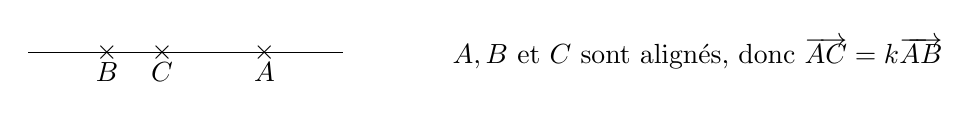
\begin{tikzpicture}
[x=0.5cm,y=0.5cm]
\draw(-4,0)--(4,0);
\draw (2,0) node[below]{$A$};
\draw (-2,0) node[below]{$B$};
\draw (-0.6,0) node[below]{$C$};
\draw (2,0) node{$\times$};
\draw (-2,0) node{$\times$};
\draw (-0.6,0) node{$\times$};
\draw (13,0) node{$A,B$ et $C$ sont alignés, donc $\overrightarrow{AC}=k\overrightarrow{AB}$};

\end{tikzpicture}
\end{center}
\end{enumerate}

\end{Propriété}

\begin{Exemple}
Dans le repère $(O,\overrightarrow{i},\overrightarrow{j})$, $A(-3;0)$, $B(-3;4)$, $C(5;0)$, $D(1;-2)$ et $E(9;-2)$.\\
Montrer que $ABCD$ est un trapèze et que les points $B,C$ et $E$ sont alignés.
\begin{center}
\begin{tikzpicture}[scale=0.8]
    % Grille en pointillés
    \draw[dotted, gray] (-5,-3) grid (10,5);
    
    % Axes principaux
    \draw[->, thick] (-5,0) -- (10,0) node[right] {$x$};
    \draw[->, thick] (0,-3) -- (0,5) node[above] {$y$};
    
    % Origine et vecteurs de base
    \node[below left] at (0,0) {$O$};
    \draw[->, thick, Couleur6] (0,0) -- (1,0) node[midway, below] {$\vec{i}$};
    \draw[->, thick, Couleur6] (0,0) -- (0,1) node[midway, left] {$\vec{j}$};
    
    % Points du parallélogramme
    \fill[Couleur8] (-3,0) circle (0pt) node[below left, Couleur8] {$A$};
    \fill[Couleur8] (-3,4) circle (0pt) node[above left, Couleur8] {$B$};
    \fill[Couleur8] (5,0) circle (0pt) node[above, Couleur8] {$C$};
    \fill[Couleur8] (1,-2) circle (0pt) node[below, Couleur8] {$D$};
    \fill[Couleur8] (9,-2) circle (0pt) node[below right, Couleur8] {$E$};
    
    % Segments du parallélogramme
    \draw[very thick, Couleur8] (-3,0) -- (-3,4); % AB
    \draw[very thick, Couleur8] (-3,4) -- (5,0);  % BC
    \draw[very thick, Couleur8] (5,0) -- (9,-2);   % CE
    \draw[very thick, Couleur8] (5,0) -- (1,-2);  % CD
    \draw[very thick, Couleur8] (1,-2) -- (-3,0); % DA
    

    
\end{tikzpicture}


\end{center}
\begin{itemize}[label=\textcolor{Couleur8}{$\bullet$}]
\item $\overrightarrow{AD}\begin{pmatrix} 
x_D-x_A \\
y_D-y_A
 \end{pmatrix}=\begin{pmatrix} 
1-(-3) \\
-2-0
 \end{pmatrix}=\begin{pmatrix} 
4 \\
-2
 \end{pmatrix}$ et  $\overrightarrow{BC}\begin{pmatrix} 
5-(-3) \\
0-4
 \end{pmatrix}=\begin{pmatrix} 
8 \\
-4
 \end{pmatrix}$. \\Donc $\overrightarrow{BC}=2\overrightarrow{AD}$ donc $\overrightarrow{BC}$ et $\overrightarrow{AD}$ sont colinéaires donc $(BC) \setminus\setminus (AD)$ donc $ABCD$ est un trapèze.
 \item $\overrightarrow{BC}\begin{pmatrix} 
8 \\
-4
 \end{pmatrix}$ et $\overrightarrow{BE}\begin{pmatrix} 
9-(-3) \\
-2-4
 \end{pmatrix}=\begin{pmatrix} 
12 \\
-6
 \end{pmatrix}$. \\
 $\det(\overrightarrow{BC};\overrightarrow{BE})=\begin{vmatrix}
8 & 12 \\
 -4 & -6
 \end{vmatrix}=8\times (-6)-(-4)\times 12=-48+48=0$.\\ Donc $\overrightarrow{BC}$ et $\overrightarrow{BE}$ sont colinéaires. Les points $B,C$ et $E$ sont donc alignés. 
 \end{itemize}
\end{Exemple}

\newpage

\section{Calculs dans un repère orthonormé}
Pour toute cette partie, on se place dans un repère {\bf{orthonormé}} $(O,\overrightarrow{i},\overrightarrow{j})$ du plan. 
\begin{Propriété}
Soit un vecteur $\overrightarrow{u}\begin{pmatrix} 
x \\
y
 \end{pmatrix}$. La norme du vecteur $\overrightarrow{u}$ est $\Vert \overrightarrow{u} \Vert=\sqrt{x^2+y^2}$.

\end{Propriété}

\begin{proof}~\\
\begin{minipage}[c]{0.65\linewidth}
Dans le repère orthonormé $(O,\overrightarrow{i},\overrightarrow{j})$, on a $\overrightarrow{u}=x\overrightarrow{i}+y\overrightarrow{j}$. \\Le théorème de Pythagore assure, dans le triangle de la figure que \\$\Vert \overrightarrow{u} \Vert ^2=x^2\Vert \overrightarrow{i} \Vert^2+y^2\Vert \overrightarrow{u} \Vert^2$. \\
Le repère étant orthonormé, $\Vert \overrightarrow{i} \Vert^2=1=\Vert \overrightarrow{j} \Vert^2$, d'où $\Vert \overrightarrow{u} \Vert ^2=x^2+y^2$.\\ Ainsi, $x^2+y^2\geq 0$, $\Vert \overrightarrow{u} \Vert=\sqrt{x^2+y^2}$.
\end{minipage} \hfill
\begin{minipage}[c]{0.35\linewidth}
\begin{center}
\begin{tikzpicture}[scale=1]
    % Grille en pointillés
    \draw[dotted, gray] (-1,-1) grid (4,3);
    
    % Axes principaux
    \draw[->, thick] (-1,0) -- (4,0) node[right] {$x$};
    \draw[->, thick] (0,-1) -- (0,3) node[above] {$y$};
    
    % Origine et vecteurs de base
    \node[below left] at (0,0) {$O$};
    \draw[->, thick, Couleur6] (0,0) -- (1,0) node[midway, below] {$\vec{i}$};
    \draw[->, thick, Couleur6] (0,0) -- (0,1) node[midway, left] {$\vec{j}$};
    
    % Vecteur u
    \draw[->, very thick, Couleur8] (0.5,0.8) -- (3.2,2.3);
    \node[above left, Couleur8] at (2,2) {$\vec{u}$};
    
    % Composantes du vecteur
    \draw[->, thick, Couleur3] (0.5,0.8) -- (3.2,0.8);
    \node[below, Couleur3] at (2,0.7) {$x\vec{i}$};
    
    \draw[->, thick, Couleur3] (3.2,0.8) -- (3.2,2.3);
    \node[right, Couleur3] at (3.2,1.5) {$y\vec{j}$};

    
\end{tikzpicture}
\end{center}

\end{minipage}

\end{proof}

\begin{Propriété}
Soient $A$ et $B$ deux points du plan.\\
La distance $AB$ est égale à la norme du vecteur $\Vert \overrightarrow{AB}\Vert$. Ainsi, $$AB=\sqrt{(x_B-x_A)^2+(y_B-y_A)^2}$$
\end{Propriété}

\begin{Exemple}
\begin{minipage}[c]{0.6\linewidth}
Soient $A(3;-2)$ et $B(2;4)$. On a :

\begin{align*}
AB &= \sqrt{(x_B-x_A)^2+(y_B-y_A)^2} \\
&= \sqrt{(2-3)^2+(4-(-2))^2} \\
&= \sqrt{(-1)^2+6^2} \\
&= \sqrt{37} \\
&\approx 6,08
\end{align*}
\end{minipage} \hfill
\begin{minipage}[c]{0.3\linewidth}
\begin{tikzpicture}[scale=0.8]
    % Grille en pointillés
    \draw[dotted, gray] (-1,-3) grid (4,5);
    
    % Axes principaux
    \draw[->, thick] (-1,0) -- (4,0) node[right] {$x$};
    \draw[->, thick] (0,-3) -- (0,5) node[above] {$y$};
    
    % Origine et vecteurs de base
    \node[below left] at (0,0) {$O$};
    \draw[->, thick, Couleur6] (0,0) -- (1,0) node[midway, below] {$\vec{i}$};
    \draw[->, thick, Couleur6] (0,0) -- (0,1) node[midway, left] {$\vec{j}$};
    
    % Points A et B
    \fill[Couleur8] (3,-2) circle (0pt) node[below right, Couleur8] {$A$};
    \fill[Couleur8] (2,4) circle (0pt) node[above left, Couleur8] {$B$};
    
    % Vecteur AB
    \draw[->, very thick, Couleur8] (3,-2) -- (2,4);

    
\end{tikzpicture}
\end{minipage}


\end{Exemple}

\begin{Propriété}
Soient $A(x_A;y_A)$ et $B(x_B;y_B)$ deux points du plan. \\
Les coordonnées du milieu $I$ du segment $[AB]$ sont $I=\left(\dfrac{x_A+x_B}{2};\dfrac{y_A+y_B}{2}\right)$.

\end{Propriété}

\begin{proof}
$I$ est le milieu de $[AB]$ donc $\overrightarrow{AI}=\overrightarrow{IB}$. On a donc, $\overrightarrow{AI}=\begin{pmatrix} 
x_I-x_A \\
y_I-y_A
 \end{pmatrix}$ et $\overrightarrow{IB}=\begin{pmatrix} 
x_B-x_I \\
y_B-y_I
 \end{pmatrix}$. \\Ces vecteurs sont égaux, donc $x_I-x_A=x_B-x_I$ et $y_I-y_A=y_B-y_I$.\\
 D'où $2x_I=x_A+x_B$ et $2y_I=y_A+y_B$. \\
~\\
 Finalement, on a bien $x_I=\dfrac{x_A+x_B}{2}$ et $y_I=\dfrac{y_A+y_B}{2} $.
\end{proof}

\newpage

\begin{Exemple}
\begin{minipage}[c]{0.65\linewidth}

Soient $A(3;-2)$ et $B(2;4)$ et $I$ le milieu de $[AB]$.\\
On a $x_I=\dfrac{x_A+x_B}{2}=\dfrac{3+2}{2}=\dfrac{5}{2}$ et $y_I=\dfrac{y_A+y_B}{2} =\dfrac{-2+4}{2}=1$.\\
Le point $I$ a donc pour coordonnées $\left(\dfrac{5}{2};1\right)$.

\end{minipage} \hfill
\begin{minipage}[c]{0.3\linewidth}
\begin{tikzpicture}[scale=0.8]
    % Grille en pointillés
    \draw[dotted, gray] (-1,-3) grid (4,5);
    
    % Axes principaux
    \draw[->, thick] (-1,0) -- (4,0) node[right] {$x$};
    \draw[->, thick] (0,-3) -- (0,5) node[above] {$y$};
    
    % Origine et vecteurs de base
    \node[below left] at (0,0) {$O$};
    \draw[->, thick, Couleur6] (0,0) -- (1,0) node[midway, below] {$\vec{i}$};
    \draw[->, thick, Couleur6] (0,0) -- (0,1) node[midway, left] {$\vec{j}$};
    
    % Points A et B
    \fill[Couleur8] (3,-2) circle (0pt) node[below right, Couleur8] {$A$};
    \fill[Couleur8] (2,4) circle (0pt) node[above left, Couleur8] {$B$};
    
    \fill[Couleur3] (2.5,1) circle (2pt) node[right, Couleur3] {$I$};
    % Vecteur AB
    \draw[->, very thick, Couleur8] (3,-2) -- (2,4);

    
\end{tikzpicture}
\end{minipage}

\end{Exemple}

\bigskip

\newpage

\section*{Exercices : Vecteurs et repérage}
\addcontentsline{toc}{section}{Exercices}
{\setlength{\columnseprule}{0pt}
\setcounter{NumEx}{1}


%https://www.melomaths.fr/static/main/pdfs/2ndCh06colinearite-fiche_exercices-corrige.pdf

\subsection*{Repérage dans le plan}


% @see : https://coopmaths.fr/alea?uuid=f71c1&id=2G24-1&n=8&d=10&s=1&alea=o9u4&cd=0&cols=1
\begin{Exercice}%1
\leavevmode\vspace{-\baselineskip}
\begin{enumerate}[itemsep=1em]
	\item \begin{minipage}[t]{\linewidth}Soit $F\left(3\,;\,2\right)$ et $G\left(4\,;\,4\right)$.Déterminer les coordonnées du vecteur $\overrightarrow{FG}$.\end{minipage}
	\item \begin{minipage}[t]{\linewidth}Soit $S\left(0\,;\,-2\right)$ et $T\left(3\,;\,-5\right)$.Déterminer les coordonnées du vecteur $\overrightarrow{ST}$.\end{minipage}
	\item \begin{minipage}[t]{\linewidth}Soit $F\left(-1\,;\,2\right)$ et $G\left(0\,;\,0\right)$.Déterminer les coordonnées du vecteur $\overrightarrow{FG}$.\end{minipage}
	\item \begin{minipage}[t]{\linewidth}Soit $T\left(1\,;\,3\right)$ et $U\left(3\,;\,0\right)$.Déterminer les coordonnées du vecteur $\overrightarrow{TU}$.\end{minipage}
	\item \begin{minipage}[t]{\linewidth}Soit $D\left(-1\,;\,2\right)$ et $E\left(1\,;\,-2\right)$.Déterminer les coordonnées du vecteur $\overrightarrow{DE}$.\end{minipage}
	\item \begin{minipage}[t]{\linewidth}Soit $F\left(3\,;\,0\right)$ et $G\left(6\,;\,4\right)$.Déterminer les coordonnées du vecteur $\overrightarrow{FG}$.\end{minipage}
	\item \begin{minipage}[t]{\linewidth}Soit $V\left(3\,;\,4\right)$ et $W\left(3\,;\,8\right)$.Déterminer les coordonnées du vecteur $\overrightarrow{VW}$.\end{minipage}
	\item \begin{minipage}[t]{\linewidth}Soit $F\left(-1\,;\,-3\right)$ et $G\left(-4\,;\,-7\right)$.Déterminer les coordonnées du vecteur $\overrightarrow{FG}$.\end{minipage}
\end{enumerate}
\end{Exercice}

% @see : https://coopmaths.fr/alea?uuid=49570&id=2G24-2&n=8&d=10&s=1&alea=R0VH&cd=0&cols=1
\begin{Exercice}%2
Soit un repère orthonormé $(O;\vec \imath, \overrightarrow{j})$. Dans chaque cas déterminer les coordonnées du vecteur $\overrightarrow{w}=\overrightarrow{u}+\overrightarrow{v}$.
\vspace{-0.5cm}
\begin{multicols}{2}
\begin{enumerate}[itemsep=1em]

	\item $\overrightarrow{u}\begin{pmatrix}-1\\6\end{pmatrix}$ et $\overrightarrow{v}\begin{pmatrix}-5\\7\end{pmatrix}$
	\item $\overrightarrow{u}\begin{pmatrix}-6\\3\end{pmatrix}$ et $\overrightarrow{v}\begin{pmatrix}9\\-2\end{pmatrix}$.
	\item $\overrightarrow{u}\begin{pmatrix}-5\\8\end{pmatrix}$ et $\overrightarrow{v}\begin{pmatrix}-4\\-4\end{pmatrix}$.
	\item $\overrightarrow{u}\begin{pmatrix}5\\9\end{pmatrix}$ et $\overrightarrow{v}\begin{pmatrix}-6\\4\end{pmatrix}$.
	\item $\overrightarrow{u}\begin{pmatrix}-3\\-1\end{pmatrix}$ et $\overrightarrow{v}\begin{pmatrix}-3\\-2\end{pmatrix}$.
	\item $\overrightarrow{u}\begin{pmatrix}-9\\-6\end{pmatrix}$ et $\overrightarrow{v}\begin{pmatrix}-4\\3\end{pmatrix}$.
	\item $\overrightarrow{u}\begin{pmatrix}0\\4\end{pmatrix}$ et $\overrightarrow{v}\begin{pmatrix}-9\\3\end{pmatrix}$.
	\item$\overrightarrow{u}\begin{pmatrix}-2\\9\end{pmatrix}$ et $\overrightarrow{v}\begin{pmatrix}-8\\-8\end{pmatrix}$.

\end{enumerate}
\end{multicols}
\end{Exercice}

% @see : https://coopmaths.fr/alea?uuid=14a2c&id=2G24-3&n=8&d=10&s=1&alea=tghZ&cd=0&cols=1
\begin{Exercice}%3
Dans chaque cas déterminer les coordonnées du vecteur $\overrightarrow{w}=\overrightarrow{u}-\overrightarrow{v}$.
\vspace{-0.5cm}
\begin{multicols}{4}
\begin{enumerate}[itemsep=1em]
\begin{small}
	\item $\vec{u}\begin{pmatrix}5\\5\end{pmatrix}$ et $\vec{v}\begin{pmatrix}-8\\-7\end{pmatrix}$.
	\item$\vec{u}\begin{pmatrix}-2\\2\end{pmatrix}$ et $\vec{v}\begin{pmatrix}5\\-3\end{pmatrix}$.
	\item $\vec{u}\begin{pmatrix}4\\5\end{pmatrix}$ et $\vec{v}\begin{pmatrix}8\\-5\end{pmatrix}$.
	\item $\vec{u}\begin{pmatrix}0\\-2\end{pmatrix}$ et $\vec{v}\begin{pmatrix}7\\3\end{pmatrix}$.
	\item $\vec{u}\begin{pmatrix}-1\\7\end{pmatrix}$ et $\vec{v}\begin{pmatrix}-6\\7\end{pmatrix}$.
	\item $\vec{u}\begin{pmatrix}0\\-8\end{pmatrix}$ et $\vec{v}\begin{pmatrix}4\\2\end{pmatrix}$.
	\item $\vec{u}\begin{pmatrix}-2\\-7\end{pmatrix}$ et $\vec{v}\begin{pmatrix}-3\\-3\end{pmatrix}$.
	\item $\vec{u}\begin{pmatrix}5\\-9\end{pmatrix}$ et $\vec{v}\begin{pmatrix}1\\-1\end{pmatrix}$.
\end{small}
\end{enumerate}
\end{multicols}
\end{Exercice}

\newpage


% @see : https://coopmaths.fr/alea?uuid=68693&id=2G24-4&n=8&d=10&s=4&alea=BqAg&cd=0&cols=1
\begin{Exercice}%4
\leavevmode\vspace{-\baselineskip}
\begin{enumerate}[itemsep=1em]
	\item \begin{minipage}[t]{\linewidth} $\overrightarrow{u}\begin{pmatrix}-7\\7\end{pmatrix}$ et $\overrightarrow{v}\begin{pmatrix}-1\\-8\end{pmatrix}$.\\Déterminer les coordonnées du vecteur $\overrightarrow{w}=\overrightarrow{u}-8\overrightarrow{v}$.\end{minipage}
	\item \begin{minipage}[t]{\linewidth} $\overrightarrow{u}\begin{pmatrix}-4\\[0.7em]-3\end{pmatrix}$ et $\overrightarrow{v}\begin{pmatrix}\dfrac{3}{5}\\[0.7em]-3\end{pmatrix}$.\\Déterminer les coordonnées du vecteur $\overrightarrow{w}=\overrightarrow{u}+\dfrac{4}{5}\overrightarrow{v}$.\end{minipage}
	\item \begin{minipage}[t]{\linewidth}Dans un repère orthonormé $(O;\vec \imath, \overrightarrow{j})$, on donne les points suivants : $A\left(4\,;\,1\right)$, $B\left(9\,;\,-8\right)$, $C\left(5\,;\,8\right)$ et $D\left(2\,;\,7\right)$.\\Déterminer les coordonnées du vecteur $\overrightarrow{w}=\overrightarrow{AB}-7\overrightarrow{CD}$.\end{minipage}
	\item \begin{minipage}[t]{\linewidth}Dans un repère orthonormé $(O;\vec \imath, \overrightarrow{j})$, on donne les points suivants : $A\left(-3\,;\,-2\right)$, $B\left(-7\,;\,-6\right)$, $C\left(-3\,;\,8\right)$ et $D\left(8\,;\,7\right)$.\\Déterminer les coordonnées du vecteur $\overrightarrow{w}=\overrightarrow{AB}+6\overrightarrow{CD}$.\end{minipage}
	\item \begin{minipage}[t]{\linewidth} $\overrightarrow{u}\begin{pmatrix}-9\\9\end{pmatrix}$ et $\overrightarrow{v}\begin{pmatrix}-1\\2\end{pmatrix}$.\\Déterminer les coordonnées du vecteur $\overrightarrow{w}=\overrightarrow{u}-7\overrightarrow{v}$.\end{minipage}
	\item \begin{minipage}[t]{\linewidth} $\overrightarrow{u}\begin{pmatrix}-1\\[0.7em]8\end{pmatrix}$ et $\overrightarrow{v}\begin{pmatrix}\dfrac{2}{3}\\[0.7em]-3\end{pmatrix}$.\\Déterminer les coordonnées du vecteur $\overrightarrow{w}=\overrightarrow{u}-\dfrac{2}{3}\overrightarrow{v}$.\end{minipage}
	\item \begin{minipage}[t]{\linewidth} $\overrightarrow{u}\begin{pmatrix}-9\\[0.7em]-8\end{pmatrix}$ et $\overrightarrow{v}\begin{pmatrix}\dfrac{1}{4}\\[0.7em]-8\end{pmatrix}$.\\Déterminer les coordonnées du vecteur $\overrightarrow{w}=\overrightarrow{u}+\dfrac{5}{2}\overrightarrow{v}$.\end{minipage}
	\item \begin{minipage}[t]{\linewidth}Dans un repère orthonormé $(O;\vec \imath, \overrightarrow{j})$, on donne les points suivants : $A\left(-2\,;\,-9\right)$, $B\left(-3\,;\,7\right)$, $C\left(8\,;\,-4\right)$ et $D\left(4\,;\,-2\right)$.\\Déterminer les coordonnées du vecteur $\overrightarrow{w}=\overrightarrow{AB}-4\overrightarrow{CD}$.\end{minipage}
\end{enumerate}
\end{Exercice}

% @see : https://coopmaths.fr/alea?uuid=222f6&id=2G24-5&n=8&d=10&s=4&alea=eLwc&cd=0&cols=1
\begin{Exercice}%5
\leavevmode\vspace{-\baselineskip}
\begin{enumerate}[itemsep=1em]
	\item \begin{minipage}[t]{\linewidth}Dans un repère orthonormé $(O;\vec \imath, \overrightarrow{j})$, on donne le point $A(6\,;\,-7)$ et le vecteur $\overrightarrow{u}\begin{pmatrix}7\\3\end{pmatrix}$.\\Déterminer les coordonnées du point $B$ tel que $\overrightarrow{u}=\overrightarrow{AB}$.\end{minipage}
	\item \begin{minipage}[t]{\linewidth}Dans un repère orthonormé $(O;\vec \imath, \overrightarrow{j})$, on donne les points $A(-7\,;\,2)$, $C(-1\,;\,-4)$, $D(-5\,;\,-8)$ et le vecteur $\overrightarrow{u}\begin{pmatrix}-6\\-5\end{pmatrix}$.\\Déterminer les coordonnées du point $B$ tel que $\overrightarrow{u}=\overrightarrow{AB}+\overrightarrow{CD}$.\end{minipage}
	\item \begin{minipage}[t]{\linewidth}Dans un repère orthonormé $(O;\vec \imath, \overrightarrow{j})$, on donne les points suivants : $A(-2;4)$, $C(8;-4)$ et $D(-5;1)$.\\Déterminer les coordonnées du point $B$ tel que $\overrightarrow{CD}=-8\overrightarrow{AB}$.\end{minipage}
	\item \begin{minipage}[t]{\linewidth}Dans un repère orthonormé $(O;\vec \imath, \overrightarrow{j})$, on donne les points suivants : $A(-5;6)$, $C(-9;-2)$ et $D(-2;-5)$.\\Déterminer les coordonnées du point $B$ tel que $\overrightarrow{CD}=5\overrightarrow{AB}$.\end{minipage}
	\item \begin{minipage}[t]{\linewidth}Dans un repère orthonormé $(O;\vec \imath, \overrightarrow{j})$, on donne les points $A(7\,;\,-4)$, $C(-9\,;\,-2)$, $D(-4\,;\,-5)$ et le vecteur $\overrightarrow{u}\begin{pmatrix}-3\\2\end{pmatrix}$.\\Déterminer les coordonnées du point $B$ tel que $\overrightarrow{u}=\overrightarrow{BA}+\overrightarrow{CD}$.\end{minipage}
	\item \begin{minipage}[t]{\linewidth}Dans un repère orthonormé $(O;\vec \imath, \overrightarrow{j})$, on donne le point $A(6\,;\,-7)$ et le vecteur $\overrightarrow{u}\begin{pmatrix}8\\-4\end{pmatrix}$.\\Déterminer les coordonnées du point $B$ tel que $\overrightarrow{u}=\overrightarrow{AB}$.\end{minipage}
	\item \begin{minipage}[t]{\linewidth}Dans un repère orthonormé $(O;\vec \imath, \overrightarrow{j})$, on donne les points $A(5\,;\,-1)$, $C(-4\,;\,1)$, $D(-5\,;\,2)$ et le vecteur $\overrightarrow{u}\begin{pmatrix}-2\\-1\end{pmatrix}$.\\Déterminer les coordonnées du point $B$ tel que $\overrightarrow{u}=\overrightarrow{BA}+\overrightarrow{CD}$.\end{minipage}
	\item \begin{minipage}[t]{\linewidth}Dans un repère orthonormé $(O;\vec \imath, \overrightarrow{j})$, on donne le point $A(2\,;\,2)$ et le vecteur $\overrightarrow{u}\begin{pmatrix}8\\3\end{pmatrix}$.\\Déterminer les coordonnées du point $B$ tel que $\overrightarrow{u}=\overrightarrow{BA}$.\end{minipage}
\end{enumerate}
\end{Exercice}

% @see : https://coopmaths.fr/alea?uuid=6b705&id=2G24-6&n=4&d=10&alea=XERh&cd=1&cols=1
\begin{Exercice}%6
\leavevmode\vspace{-\baselineskip}
\begin{enumerate}[itemsep=1em]
	\item \begin{minipage}[t]{\linewidth}Dans un repère $(O\;;\;\overrightarrow{i}\;;\;\overrightarrow{j})$, on considère les points $A(3\;;\;-3)$, $B(0\;;\;7)$ et $C(9\;;\;-8)$.\\Déterminer les coordonnées du point $D$ tel que $ABCD$ soit un parallélogramme.\end{minipage}
	\item \begin{minipage}[t]{\linewidth}Dans un repère $(O\;;\;\overrightarrow{i}\;;\;\overrightarrow{j})$, on considère les points $C(8\;;\;-10)$, $D(-3\;;\;-5)$ et $E(-1\;;\;5)$.\\Déterminer les coordonnées du point $F$ tel que $CDEF$ soit un parallélogramme.\end{minipage}
	\item \begin{minipage}[t]{\linewidth}Dans un repère $(O\;;\;\overrightarrow{i}\;;\;\overrightarrow{j})$, on considère les points $W(8\;;\;1)$, $X(-6\;;\;4)$ et $Y(-4\;;\;9)$.\\Déterminer les coordonnées du point $Z$ tel que $WXYZ$ soit un parallélogramme.\end{minipage}
	\item \begin{minipage}[t]{\linewidth}Dans un repère $(O\;;\;\overrightarrow{i}\;;\;\overrightarrow{j})$, on considère les points $D(10\;;\;-6)$, $E(-7\;;\;-8)$ et $F(7\;;\;0)$.\\Déterminer les coordonnées du point $G$ tel que $DEFG$ soit un parallélogramme.\end{minipage}
\end{enumerate}
\end{Exercice}


\subsection*{Colinéarité}
\begin{Exercice}
Soient A(4;-3), B(-1;5), C(-3;1) et D(7;-15).
Les vecteurs $ \overrightarrow{AB} $ et $ \overrightarrow{CD} $ sont-ils colinéaires ?
\end{Exercice}


\begin{Exercice}
Soient A(-3;5), B(-6;-1), C(8;2) et D(-1;-16).
Les vecteurs $ \overrightarrow{AB} $ et $ \overrightarrow{CD} $ sont-ils colinéaires ?
\end{Exercice}



\begin{Exercice}
Soient A(-1;4), B(-4;2), C(7;-2) et D(-2;-8).
Les vecteurs $ \overrightarrow{AB} $ et $ \overrightarrow{CD} $ sont-ils colinéaires ?
\end{Exercice}

\newpage

\begin{Exercice}
Dans chaque cas, démontrer que les vecteurs $ \overrightarrow{AB} $ et $ \overrightarrow{CD} $ sont colinéaires.
\vspace{-0.5cm}
\begin{multicols}{3}
\begin{enumerate}
\item $ 4\overrightarrow{AD} -4\overrightarrow{BD} +2\overrightarrow{CD} = 0 $
\item $ \overrightarrow{CB}+2\overrightarrow{AC} + \overrightarrow{DB} = 0 $
\item $ 5\overrightarrow{AB}-3\overrightarrow{CB} = 7\overrightarrow{AD}-4\overrightarrow{AC} $
\end{enumerate}
\end{multicols}
\end{Exercice}

\begin{Exercice}
Dans chacun des cas, calculer le déterminant de $ \overrightarrow{u} $ et $ \overrightarrow{v} $.
\vspace{-0.5cm}
\begin{multicols}{2}
\begin{enumerate}
\item  $ \overrightarrow{u}(1;5) $ et $ \overrightarrow{v}(2;7) $
\item $ \overrightarrow{u}(-3;4) $ et $  \overrightarrow{v}(8;11) $.
\item $ \overrightarrow{u}(2;6) $ et $ \overrightarrow{v}(-6;-18) $.
\item $ \overrightarrow{u}(-2;1) $ et $ \overrightarrow{v} \left(  \dfrac{1}{3};4 \right)   $.
\end{enumerate}
\end{multicols}
\end{Exercice}



\begin{Exercice}
Dans chaque cas, dire si les vecteurs $ \overrightarrow{u} $ et $ \overrightarrow{v} $ sont colinéaires.
\vspace{-0.5cm}
\begin{multicols}{2}
\begin{enumerate}
\item $ \overrightarrow{u}(4;7) $ et $ \overrightarrow{v}(-2;5) $.
\item $ \overrightarrow{u}(-2;5) $ et $ \overrightarrow{v}(-5;12,5) $.
\item $ \overrightarrow{u}\left( \dfrac{1}{2};-4\right)  $ et $ \overrightarrow{v}(-6;48) $.
\item $ \overrightarrow{u}\left( \dfrac{1}{3};2\right)  $ et $ \overrightarrow{v}(-2;6) $.
\end{enumerate}
\end{multicols}
\end{Exercice}


\begin{Exercice}
Dans chaque cas, déterminer le nombre réel $ m $ pour que les vecteurs $ \overrightarrow{u} $ et $ \overrightarrow{v} $ soient colinéaires.
\vspace{-0.5cm}
\begin{multicols}{2}
\begin{enumerate}
\item $ \overrightarrow{u}(3;-1) $ et $ \overrightarrow{v}(m;54) $.
\item $ \overrightarrow{u}(2m;-5) $ et $ \overrightarrow{v}(m;-1) $.
\end{enumerate}
\end{multicols}
\end{Exercice}



% @see : https://coopmaths.fr/alea?uuid=b1777&id=2G33-1&n=6&d=10&s=1&alea=wbLv&cd=1&cols=2
\begin{Exercice}
Soit $\big(O,\vec i;\vec j\big)$ un repère orthogonal.  Déterminer si les 3 points $A$, $B$ et $C$ suivants sont ou non alignés.
\vspace{-0.5cm}
\begin{multicols}{2}
\begin{enumerate}[itemsep=1em]
	\item \begin{minipage}[t]{\linewidth} $A(-1;0)$ ; $B(4;-4)$ et $C(-11;8)$.\end{minipage}
	\item \begin{minipage}[t]{\linewidth} $A(-4;5)$ ; $B(-2;-5)$ et $C(-5;3)$.\end{minipage}
	\item \begin{minipage}[t]{\linewidth} $A(0;-2)$ ; $B(-4;4)$ et $C(4;-8)$.\end{minipage}
	\item \begin{minipage}[t]{\linewidth} $A(1;0)$ ; $B(-3;-5)$ et $C(3;2)$.\end{minipage}
	\item \begin{minipage}[t]{\linewidth} $A(-1;2)$ ; $B(1;-4)$ et $C(-5;14)$.\end{minipage}
	\item \begin{minipage}[t]{\linewidth} $A(-5;-1)$ ; $B(5;2)$ et $C(1;-2)$.\end{minipage}
\end{enumerate}
\end{multicols}
\end{Exercice}


\begin{Exercice}
Dans un repère, on donne les points :
\begin{center}
A(1;-1); B(4;2) et C(-2;5)
\end{center}
D est le point tel que $ \overrightarrow{CD} = \dfrac{1}{3}\overrightarrow{BA} + \dfrac{2}{3}\overrightarrow{CA} $.
\begin{enumerate}
	\item Déterminer les coordonnées du point D.
	\item Émettre une conjecture pour les droites (BC) et (AD).
	\item Démontrer cette conjecture
\end{enumerate}
\end{Exercice}



\begin{Exercice}
 Dans un repère, on donne les points :
\begin{center}
A(3;4); B(2;1) et C(6;1)
\end{center}
D est le point tel que $ \overrightarrow{AD} = 2\overrightarrow{AB}-\overrightarrow{BC} $
E est le symétrique de C par rapport à B.
\begin{enumerate}
	\item Émettre une conjecture pour les droites (AB) et (DE).
	\item Démontrer cette conjecture
\end{enumerate}
\end{Exercice}

\begin{Exercice}
 Dans un repère, on donne les points :
\begin{center}
A(1;-1), B(2;1), C(4;-1) et D(6;-2)
\end{center}
\begin{enumerate}
	\item Placer le point E tel que $ \overrightarrow{AE} = \dfrac{3}{2}\overrightarrow{BC} $.
	\item Calculer les coordonnées du point E.
	\item Placer le point F tel que $ \overrightarrow{CF} = -3\overrightarrow{AB}$.
	\item Calculer les coordonnées du point F.
	\item Les points D, E et F sont-ils alignés?
\end{enumerate}
\end{Exercice}


\begin{Exercice}
Dans un repère, on donne les points :
\begin{center}
$ A\left(- \dfrac{7}{2};- \dfrac{1}{2} \right)  $, $ B\left( \dfrac{1}{2};\dfrac{3}{2} \right)  $ et $ C\left( \dfrac{5}{2};\dfrac{5}{2} \right)  $
\end{center}
\begin{enumerate}
	\item\begin{enumerate}
	\item Placer les point A,B, et C dans un repère.
\item Que peut-on conjecturer pour ces trois points?
\item Démontrer cette conjecture.
\end{enumerate}
\item On donne les points :
\begin{center}
$ D\left( 100; \dfrac{205}{4}\right)  $ et $ E\left( -100; -\dfrac{95}{2}\right)  $
\end{center}
Ces points sont-ils alignés avec A et B?
\end{enumerate}
\end{Exercice}

\begin{Exercice}
Dans un repère, on donne les points :
$ A(1;2) $; $ B(-3;0) $ et $ C(-14;a) $, avec $ a \in \R $.
\begin{enumerate}
	\item Exprimer les coordonnées du vecteur $ \overrightarrow{BC} $ en fonction de a.
	\item Déterminer la valeur de $ a $ pour laquelle les points A, B et C sont alignés.

\end{enumerate}
\end{Exercice}

\newpage

\subsection*{Calculs dans un repère orthonormé}

\begin{Exercice}
Dans un repère \((O,\vec{i},\vec{j})\) quelconque, on place les points \(A(2;7)\), \(B(3;-1)\), \(C(4;-3)\) et \(D(5;0)\). \\
Déterminer les coordonnées des points \(I, J, K\) et \(L\), milieux respectifs de \([AB]\), \([BC]\), \([CD]\) et \([DA]\).
\end{Exercice}

\begin{Exercice}
Dans un repère \((O,\vec{i},\vec{j})\) quelconque, on place les points \(A(5;3)\), \(B(2;4)\), \(C(-2;-3)\) et \(D(0;-2)\).

\begin{enumerate}
    \item Déterminer les coordonnées des points \(I, J, K, L\), milieux respectifs de \([AB]\), \([BC]\), \([CD]\) et \([DA]\).
    \item Montrer que \(IJKL\) est un parallélogramme.
\end{enumerate}
\end{Exercice}

\begin{Exercice}
Dans un repère \((O,\vec{i},\vec{j})\) quelconque, on place \(A(5;3)\) et \(I(2;-1)\). \\
Déterminer les coordonnées du point \(B\) tel que \(I\) soit le milieu de \([AB]\).
\end{Exercice}

\begin{Exercice}
Dans un repère \((O,\vec{i},\vec{j})\) quelconque, le point \(M\) a pour abscisse 2 et le point \(N\) a pour ordonnée -3. \\
Le point \(I\) de coordonnées (5;1) est le milieu de \([MN]\).\\
 Déterminer les coordonnées de \(M\) et \(N\).
\end{Exercice}

\begin{Exercice}
Dans un repère \((O,\vec{i},\vec{j})\) orthonormé, on place les points \(A(5;3)\), \(B(2;4)\), \(C(-2;-3)\). \\
Calculer les distances \(AB\), \(BC\) et \(AC\).
\end{Exercice}

\begin{Exercice}
Dans un repère \((O,\vec{i},\vec{j})\) orthonormé, on place les points \(D(1;4)\), \(E(5;2)\), \(F(1;-1)\). \\
Montrer que le triangle \(DEF\) est isocèle.
\end{Exercice}

\begin{Exercice}
Dans un repère \((O,\vec{i},\vec{j})\) orthonormé, on place les points \(G(3;3)\), \(H(5;2)\), \(I(0;-3)\). \\
Montrer que le triangle \(GHI\) est rectangle en \(G\).
\end{Exercice}

\begin{Exercice}
Dans un repère \((O,\vec{i},\vec{j})\) orthonormé, on place les points \(J(-3;3)\), \(K(-4;1)\), \(L(0;-1)\) et \(M(1;1)\).\\
 Montrer que le quadrilatère \(JKLM\) est un rectangle.
\end{Exercice}

\begin{Exercice}
Dans un repère \((O,\vec{i},\vec{j})\) orthonormé, on place les points \(P(-2;0)\), \(Q(4;2)\) et \(R(0;4)\).

\begin{enumerate}
    \item Montrer que le triangle \(PQR\) est isocèle et rectangle en \(R\).
    \item Déterminer les coordonnées de \(I\), milieu de \([PQ]\).
    \item Montrer que \(IQ = IP = IR\).
\end{enumerate}
\end{Exercice}


}
